% Created by tikzDevice version 0.10.1 on 2016-08-23 15:31:27
% !TEX encoding = UTF-8 Unicode
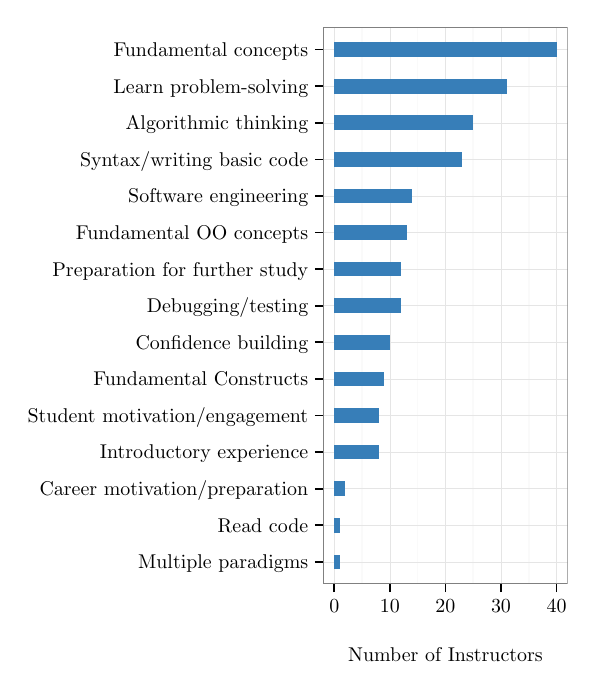
\begin{tikzpicture}[x=1pt,y=1pt]
\definecolor{fillColor}{RGB}{255,255,255}
\path[use as bounding box,fill=fillColor,fill opacity=0.00] (0,0) rectangle (195.13,231.26);
\begin{scope}
\path[clip] (  0.00,  0.00) rectangle (195.13,231.26);
\definecolor{drawColor}{RGB}{255,255,255}
\definecolor{fillColor}{RGB}{255,255,255}

\path[draw=drawColor,line width= 0.6pt,line join=round,line cap=round,fill=fillColor] (  0.00,  0.00) rectangle (195.13,231.26);
\end{scope}
\begin{scope}
\path[clip] (106.78, 30.29) rectangle (195.13,231.26);
\definecolor{fillColor}{RGB}{255,255,255}

\path[fill=fillColor] (106.78, 30.29) rectangle (195.13,231.26);
\definecolor{drawColor}{gray}{0.98}

\path[draw=drawColor,line width= 0.6pt,line join=round] (120.83, 30.29) --
	(120.83,231.26);

\path[draw=drawColor,line width= 0.6pt,line join=round] (140.91, 30.29) --
	(140.91,231.26);

\path[draw=drawColor,line width= 0.6pt,line join=round] (160.99, 30.29) --
	(160.99,231.26);

\path[draw=drawColor,line width= 0.6pt,line join=round] (181.07, 30.29) --
	(181.07,231.26);
\definecolor{drawColor}{gray}{0.90}

\path[draw=drawColor,line width= 0.2pt,line join=round] (106.78, 38.23) --
	(195.13, 38.23);

\path[draw=drawColor,line width= 0.2pt,line join=round] (106.78, 51.45) --
	(195.13, 51.45);

\path[draw=drawColor,line width= 0.2pt,line join=round] (106.78, 64.67) --
	(195.13, 64.67);

\path[draw=drawColor,line width= 0.2pt,line join=round] (106.78, 77.89) --
	(195.13, 77.89);

\path[draw=drawColor,line width= 0.2pt,line join=round] (106.78, 91.11) --
	(195.13, 91.11);

\path[draw=drawColor,line width= 0.2pt,line join=round] (106.78,104.34) --
	(195.13,104.34);

\path[draw=drawColor,line width= 0.2pt,line join=round] (106.78,117.56) --
	(195.13,117.56);

\path[draw=drawColor,line width= 0.2pt,line join=round] (106.78,130.78) --
	(195.13,130.78);

\path[draw=drawColor,line width= 0.2pt,line join=round] (106.78,144.00) --
	(195.13,144.00);

\path[draw=drawColor,line width= 0.2pt,line join=round] (106.78,157.22) --
	(195.13,157.22);

\path[draw=drawColor,line width= 0.2pt,line join=round] (106.78,170.44) --
	(195.13,170.44);

\path[draw=drawColor,line width= 0.2pt,line join=round] (106.78,183.67) --
	(195.13,183.67);

\path[draw=drawColor,line width= 0.2pt,line join=round] (106.78,196.89) --
	(195.13,196.89);

\path[draw=drawColor,line width= 0.2pt,line join=round] (106.78,210.11) --
	(195.13,210.11);

\path[draw=drawColor,line width= 0.2pt,line join=round] (106.78,223.33) --
	(195.13,223.33);

\path[draw=drawColor,line width= 0.2pt,line join=round] (110.79, 30.29) --
	(110.79,231.26);

\path[draw=drawColor,line width= 0.2pt,line join=round] (130.87, 30.29) --
	(130.87,231.26);

\path[draw=drawColor,line width= 0.2pt,line join=round] (150.95, 30.29) --
	(150.95,231.26);

\path[draw=drawColor,line width= 0.2pt,line join=round] (171.03, 30.29) --
	(171.03,231.26);

\path[draw=drawColor,line width= 0.2pt,line join=round] (191.11, 30.29) --
	(191.11,231.26);
\definecolor{fillColor}{RGB}{55,126,184}

\path[fill=fillColor] (110.79, 35.58) rectangle (112.80, 40.87);

\path[fill=fillColor] (110.79, 48.80) rectangle (112.80, 54.09);

\path[fill=fillColor] (110.79, 62.03) rectangle (114.81, 67.31);

\path[fill=fillColor] (110.79, 75.25) rectangle (126.86, 80.54);

\path[fill=fillColor] (110.79, 88.47) rectangle (126.86, 93.76);

\path[fill=fillColor] (110.79,101.69) rectangle (128.86,106.98);

\path[fill=fillColor] (110.79,114.91) rectangle (130.87,120.20);

\path[fill=fillColor] (110.79,128.13) rectangle (134.89,133.42);

\path[fill=fillColor] (110.79,141.36) rectangle (134.89,146.64);

\path[fill=fillColor] (110.79,154.58) rectangle (136.90,159.87);

\path[fill=fillColor] (110.79,167.80) rectangle (138.90,173.09);

\path[fill=fillColor] (110.79,181.02) rectangle (156.98,186.31);

\path[fill=fillColor] (110.79,194.24) rectangle (160.99,199.53);

\path[fill=fillColor] (110.79,207.46) rectangle (173.04,212.75);

\path[fill=fillColor] (110.79,220.69) rectangle (191.11,225.98);
\definecolor{drawColor}{gray}{0.50}

\path[draw=drawColor,line width= 0.6pt,line join=round,line cap=round] (106.78, 30.29) rectangle (195.13,231.26);
\end{scope}
\begin{scope}
\path[clip] (  0.00,  0.00) rectangle (195.13,231.26);
\definecolor{drawColor}{RGB}{0,0,0}

\node[text=drawColor,anchor=base east,inner sep=0pt, outer sep=0pt, scale=  0.72] at (101.38, 35.75) {Multiple paradigms};

\node[text=drawColor,anchor=base east,inner sep=0pt, outer sep=0pt, scale=  0.72] at (101.38, 48.97) {Read code};

\node[text=drawColor,anchor=base east,inner sep=0pt, outer sep=0pt, scale=  0.72] at (101.38, 62.19) {Career motivation/preparation};

\node[text=drawColor,anchor=base east,inner sep=0pt, outer sep=0pt, scale=  0.72] at (101.38, 75.41) {Introductory experience};

\node[text=drawColor,anchor=base east,inner sep=0pt, outer sep=0pt, scale=  0.72] at (101.38, 88.63) {Student motivation/engagement};

\node[text=drawColor,anchor=base east,inner sep=0pt, outer sep=0pt, scale=  0.72] at (101.38,101.86) {Fundamental Constructs};

\node[text=drawColor,anchor=base east,inner sep=0pt, outer sep=0pt, scale=  0.72] at (101.38,115.08) {Confidence building};

\node[text=drawColor,anchor=base east,inner sep=0pt, outer sep=0pt, scale=  0.72] at (101.38,128.30) {Debugging/testing};

\node[text=drawColor,anchor=base east,inner sep=0pt, outer sep=0pt, scale=  0.72] at (101.38,141.52) {Preparation for further study};

\node[text=drawColor,anchor=base east,inner sep=0pt, outer sep=0pt, scale=  0.72] at (101.38,154.74) {Fundamental OO concepts};

\node[text=drawColor,anchor=base east,inner sep=0pt, outer sep=0pt, scale=  0.72] at (101.38,167.96) {Software engineering};

\node[text=drawColor,anchor=base east,inner sep=0pt, outer sep=0pt, scale=  0.72] at (101.38,181.19) {Syntax/writing basic code};

\node[text=drawColor,anchor=base east,inner sep=0pt, outer sep=0pt, scale=  0.72] at (101.38,194.41) {Algorithmic thinking};

\node[text=drawColor,anchor=base east,inner sep=0pt, outer sep=0pt, scale=  0.72] at (101.38,207.63) {Learn problem-solving};

\node[text=drawColor,anchor=base east,inner sep=0pt, outer sep=0pt, scale=  0.72] at (101.38,220.85) {Fundamental concepts};
\end{scope}
\begin{scope}
\path[clip] (  0.00,  0.00) rectangle (195.13,231.26);
\definecolor{drawColor}{RGB}{0,0,0}

\path[draw=drawColor,line width= 0.6pt,line join=round] (103.78, 38.23) --
	(106.78, 38.23);

\path[draw=drawColor,line width= 0.6pt,line join=round] (103.78, 51.45) --
	(106.78, 51.45);

\path[draw=drawColor,line width= 0.6pt,line join=round] (103.78, 64.67) --
	(106.78, 64.67);

\path[draw=drawColor,line width= 0.6pt,line join=round] (103.78, 77.89) --
	(106.78, 77.89);

\path[draw=drawColor,line width= 0.6pt,line join=round] (103.78, 91.11) --
	(106.78, 91.11);

\path[draw=drawColor,line width= 0.6pt,line join=round] (103.78,104.34) --
	(106.78,104.34);

\path[draw=drawColor,line width= 0.6pt,line join=round] (103.78,117.56) --
	(106.78,117.56);

\path[draw=drawColor,line width= 0.6pt,line join=round] (103.78,130.78) --
	(106.78,130.78);

\path[draw=drawColor,line width= 0.6pt,line join=round] (103.78,144.00) --
	(106.78,144.00);

\path[draw=drawColor,line width= 0.6pt,line join=round] (103.78,157.22) --
	(106.78,157.22);

\path[draw=drawColor,line width= 0.6pt,line join=round] (103.78,170.44) --
	(106.78,170.44);

\path[draw=drawColor,line width= 0.6pt,line join=round] (103.78,183.67) --
	(106.78,183.67);

\path[draw=drawColor,line width= 0.6pt,line join=round] (103.78,196.89) --
	(106.78,196.89);

\path[draw=drawColor,line width= 0.6pt,line join=round] (103.78,210.11) --
	(106.78,210.11);

\path[draw=drawColor,line width= 0.6pt,line join=round] (103.78,223.33) --
	(106.78,223.33);
\end{scope}
\begin{scope}
\path[clip] (  0.00,  0.00) rectangle (195.13,231.26);
\definecolor{drawColor}{RGB}{0,0,0}

\path[draw=drawColor,line width= 0.6pt,line join=round] (110.79, 27.29) --
	(110.79, 30.29);

\path[draw=drawColor,line width= 0.6pt,line join=round] (130.87, 27.29) --
	(130.87, 30.29);

\path[draw=drawColor,line width= 0.6pt,line join=round] (150.95, 27.29) --
	(150.95, 30.29);

\path[draw=drawColor,line width= 0.6pt,line join=round] (171.03, 27.29) --
	(171.03, 30.29);

\path[draw=drawColor,line width= 0.6pt,line join=round] (191.11, 27.29) --
	(191.11, 30.29);
\end{scope}
\begin{scope}
\path[clip] (  0.00,  0.00) rectangle (195.13,231.26);
\definecolor{drawColor}{RGB}{0,0,0}

\node[text=drawColor,anchor=base,inner sep=0pt, outer sep=0pt, scale=  0.72] at (110.79, 19.93) {0};

\node[text=drawColor,anchor=base,inner sep=0pt, outer sep=0pt, scale=  0.72] at (130.87, 19.93) {10};

\node[text=drawColor,anchor=base,inner sep=0pt, outer sep=0pt, scale=  0.72] at (150.95, 19.93) {20};

\node[text=drawColor,anchor=base,inner sep=0pt, outer sep=0pt, scale=  0.72] at (171.03, 19.93) {30};

\node[text=drawColor,anchor=base,inner sep=0pt, outer sep=0pt, scale=  0.72] at (191.11, 19.93) {40};
\end{scope}
\begin{scope}
\path[clip] (  0.00,  0.00) rectangle (195.13,231.26);
\definecolor{drawColor}{RGB}{0,0,0}

\node[text=drawColor,anchor=base,inner sep=0pt, outer sep=0pt, scale=  0.72] at (150.95, 10.18) {};

\node[text=drawColor,anchor=base,inner sep=0pt, outer sep=0pt, scale=  0.72] at (150.95,  2.40) {Number of Instructors};
\end{scope}
\end{tikzpicture}
